% ---
% Este capítulo, apresenta os anexos
% ---

\chapter{Resultados}
\label{chap:anexos}

\begin{table}[htb]
	\begin{tabular}{|c|c|c|c|c|}
		\hline
		\textbf{Cromossomo} 	& \textbf{Avaliação} 	& \textbf{\(\mathcal{H}(\sigma) \)}	& \textbf{Taxa de seleção}	& \textbf{Proporção estimada} \\
		\hline
		287	&  222	&  42 	&  0,067	&  0,040 \\ \hline 
		277	&  206	&  26 	&  0,050	&  0,037 \\ \hline 
		280	&  204	&  24 	&  0,033	&  0,037 \\ \hline 
		282	&  204	&  24 	&  0,017	&  0,037 \\ \hline 
		285	&  200	&  20 	&  0,000	&  0,036 \\ \hline 
		276	&  194	&  14 	&  0,000	&  0,035 \\ \hline 
		291	&  194	&  14 	&  0,083	&  0,035 \\ \hline 
		286	&  192	&  12 	&  0,017	&  0,034 \\ \hline 
		293	&  192	&  12 	&  0,033	&  0,034 \\ \hline 
		283	&  190	&  10 	&  0,033	&  0,034 \\ \hline 
		288	&  190	&  10 	&  0,017	&  0,034 \\ \hline 
		289	&  190	&  10 	&  0,000	&  0,034 \\ \hline 
		299	&  188	&  8 	&  0,017	&  0,034 \\ \hline 
		273	&  186	&  6 	&  0,067	&  0,033 \\ \hline 
		300	&  186	&  6 	&  0,017	&  0,033 \\ \hline 
		292	&  184	&  4 	&  0,033	&  0,033 \\ \hline 
		274	&  182	&  2 	&  0,000	&  0,033 \\ \hline 
		297	&  182	&  2 	&  0,067	&  0,033 \\ \hline 
		271	&  180	&  0 	&  0,033	&  0,032 \\ \hline 
		281	&  180	&  0 	&  0,033	&  0,032 \\ \hline 
		295	&  180	&  0 	&  0,050	&  0,032 \\ \hline 
		290	&  178	&  -2 	&  0,050	&  0,032 \\ \hline 
		294	&  178	&  -2 	&  0,033	&  0,032 \\ \hline 
		278	&  176	&  -4 	&  0,017	&  0,032 \\ \hline 
		284	&  176	&  -4 	&  0,067	&  0,032 \\ \hline 
		279	&  174	&  -6 	&  0,033	&  0,031 \\ \hline 
		275	&  172	&  -8 	&  0,067	&  0,031 \\ \hline 
		298	&  172	&  -8 	&  0,033	&  0,031 \\ \hline 
		272	&  164	&  -16 	&  0,000	&  0,029 \\ \hline 
		296	&  160	&  -20 	&  0,033	&  0,029 \\
		\hline
	\end{tabular}
	\caption{Resumo da geração 9 com média de avaliação 185,86 mostrando a taxa de amostragem da seleção e o que era esperado para a proporção usando a função de avaliação da \autoref{eq:Energia_modelo_ising}}
	\label{tab:resumo_GA_H}
\end{table}

\begin{table}[htb]
	\begin{tabular}{|c|c|c|c|c|}
		\hline
		\textbf{Cromossomo} 	& \textbf{Avaliação} 	& \textbf{\(\mathcal{H}(\sigma) \)}	& \textbf{Taxa de seleção}	& \textbf{Proporção estimada} \\
		\hline
		178	&  6,69		&  -38 &  0,100	&  0,063\\ \hline
		160	&  6,05		&  -36 &  0,100	&  0,057\\ \hline
		159	&  5,47		&  -34 &  0,033	&  0,052\\ \hline
		166	&  5,47		&  -34 &  0,067	&  0,052\\ \hline
		162	&  4,95		&  -32 &  0,067	&  0,047\\ \hline
		171	&  4,95		&  -32 &  0,000	&  0,047\\ \hline
		180	&  4,95		&  -32 &  0,033	&  0,047\\ \hline
		167	&  4,48		&  -30 &  0,050	&  0,042\\ \hline
		175	&  4,48		&  -30 &  0,017	&  0,042\\ \hline
		161	&  4,06		&  -28 &  0,050	&  0,038\\ \hline
		163	&  4,06		&  -28 &  0,033	&  0,038\\ \hline
		169	&  4,06		&  -28 &  0,017	&  0,038\\ \hline
		151	&  3,67		&  -26 &  0,050	&  0,035\\ \hline
		155	&  3,67		&  -26 &  0,033	&  0,035\\ \hline
		170	&  3,32		&  -24 &  0,017	&  0,031\\ \hline
		176	&  3,32		&  -24 &  0,050	&  0,031\\ \hline
		153	&  3,00		&  -22 &  0,067	&  0,028\\ \hline
		157	&  3,00		&  -22 &  0,033	&  0,028\\ \hline
		174	&  3,00		&  -22 &  0,050	&  0,028\\ \hline
		152	&  2,72		&  -20 &  0,000	&  0,026\\ \hline
		164	&  2,72		&  -20 &  0,050	&  0,026\\ \hline
		165	&  2,72		&  -20 &  0,000	&  0,026\\ \hline
		158	&  2,46		&  -18 &  0,017	&  0,023\\ \hline
		154	&  2,23		&  -16 &  0,033	&  0,021\\ \hline
		168	&  2,01		&  -14 &  0,000	&  0,019\\ \hline
		173	&  2,01		&  -14 &  0,000	&  0,019\\ \hline
		156	&  1,82		&  -12 &  0,033	&  0,017\\ \hline
		179	&  1,82		&  -12 &  0,000	&  0,017\\ \hline
		172	&  1,22		&  -4 &  0,000	&  0,012\\ \hline
		177	&  1,11		&  -2 &  0,000	&  0,010\\
		\hline
	\end{tabular}
	\caption{Resumo da geração 5 com média de avaliação 3.516 mostrando a taxa de amostragem da seleção e o que era esperado para a proporção usando a função de avaliação da \autoref{eq:selecao_modelo_ising}}
	\label{tab:resumo_GA_expH}
\end{table}

\begin{figure}[ht]
	\centering
	\begin{subfigure}[b]{0.47\linewidth}
		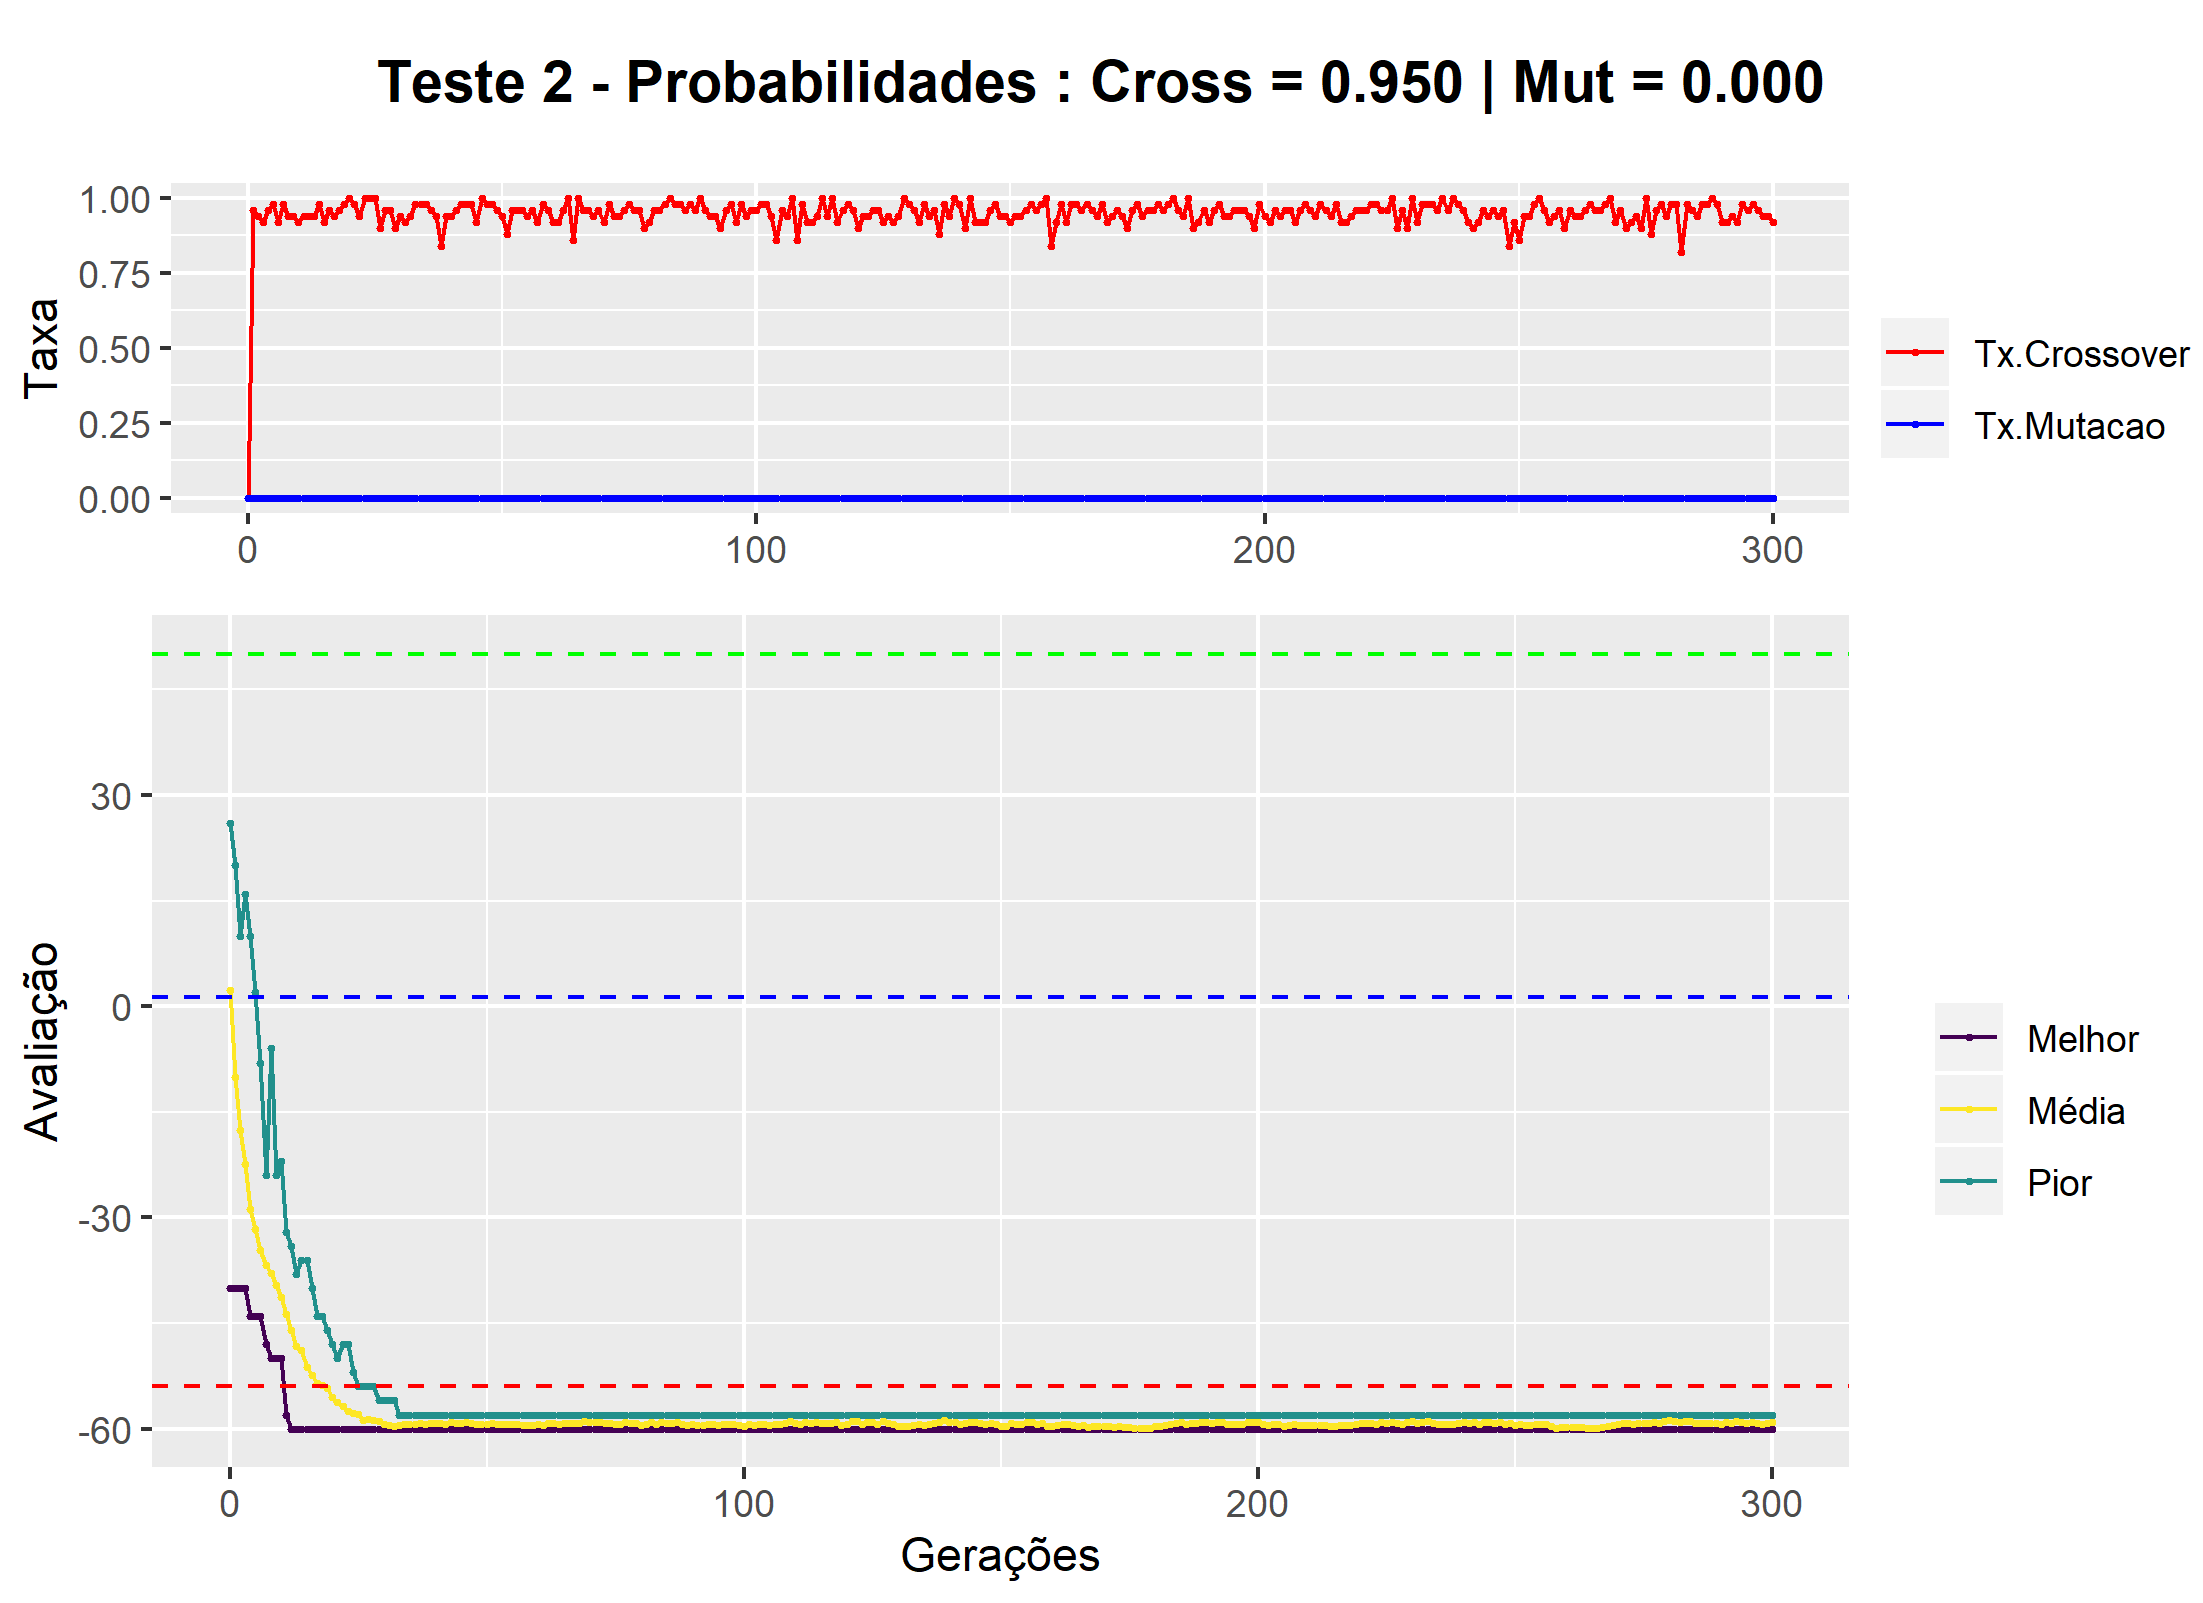
\includegraphics[width=\linewidth]{imagens/graph_pc_0_950_pm_0_000_pop_50_g_300__2.png}
		\caption{}
	\end{subfigure}
	\begin{subfigure}[b]{0.47\linewidth}
		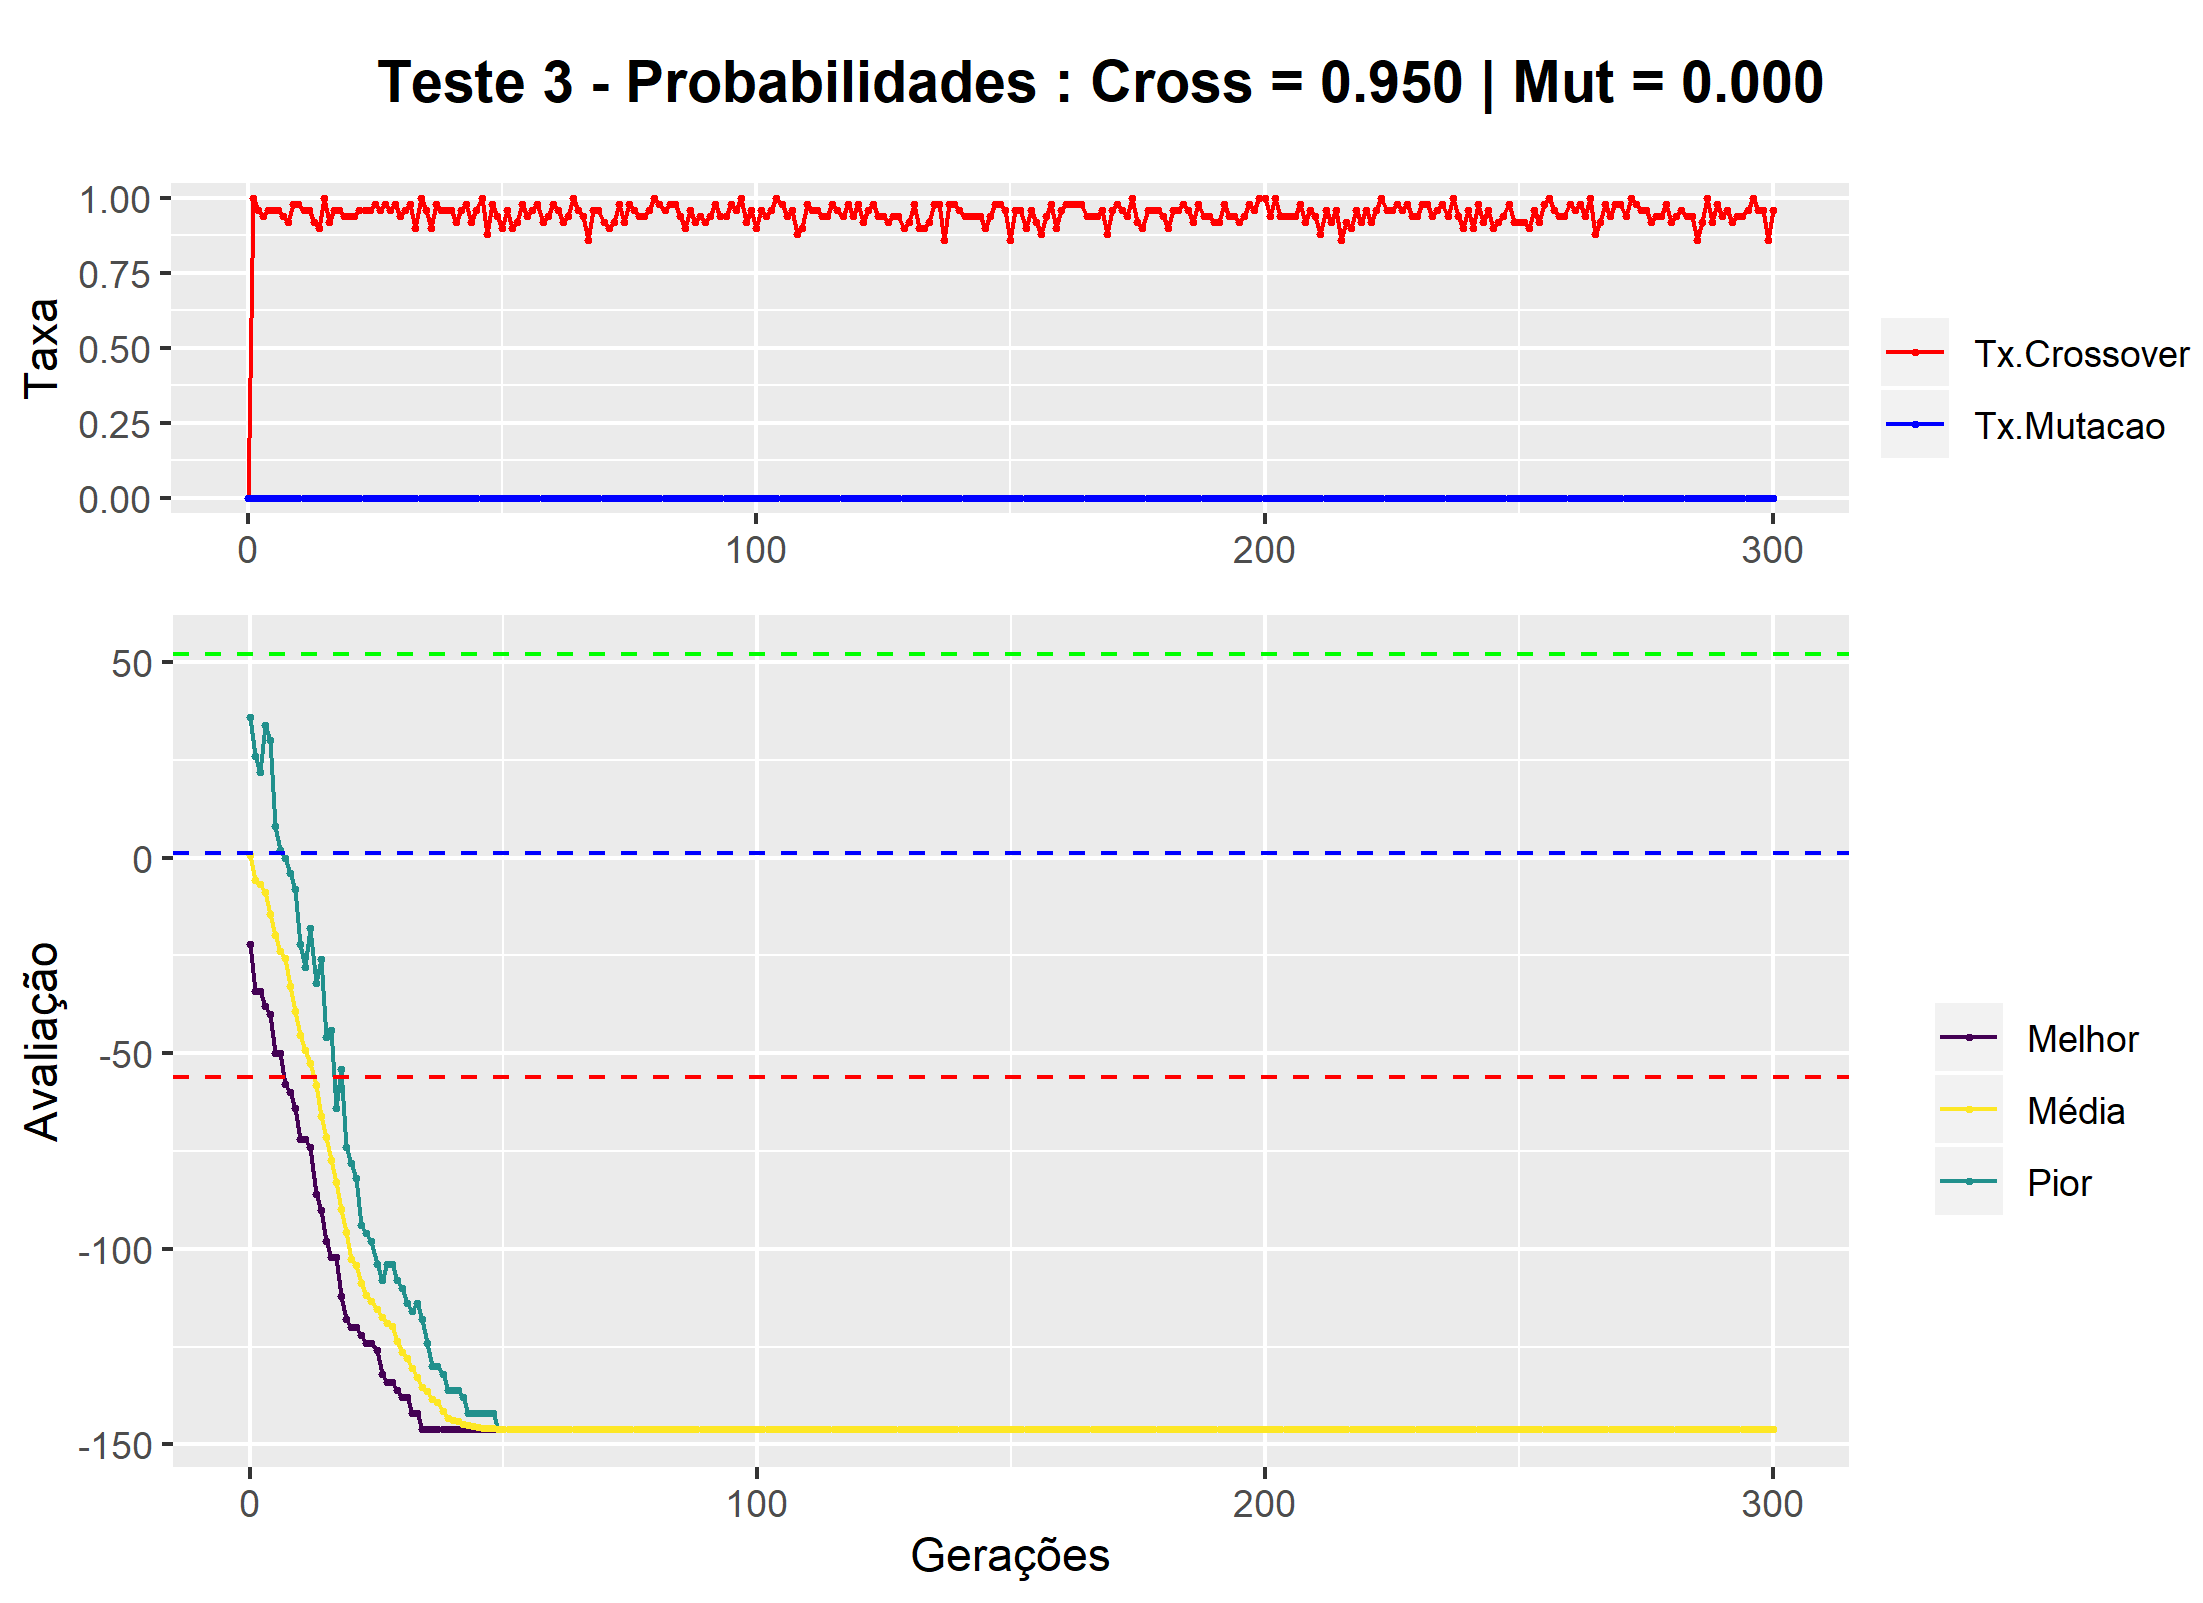
\includegraphics[width=\linewidth]{imagens/graph_pc_0_950_pm_0_000_pop_50_g_300__3.png}
		\caption{}
	\end{subfigure}
	\begin{subfigure}[b]{0.47\linewidth}
		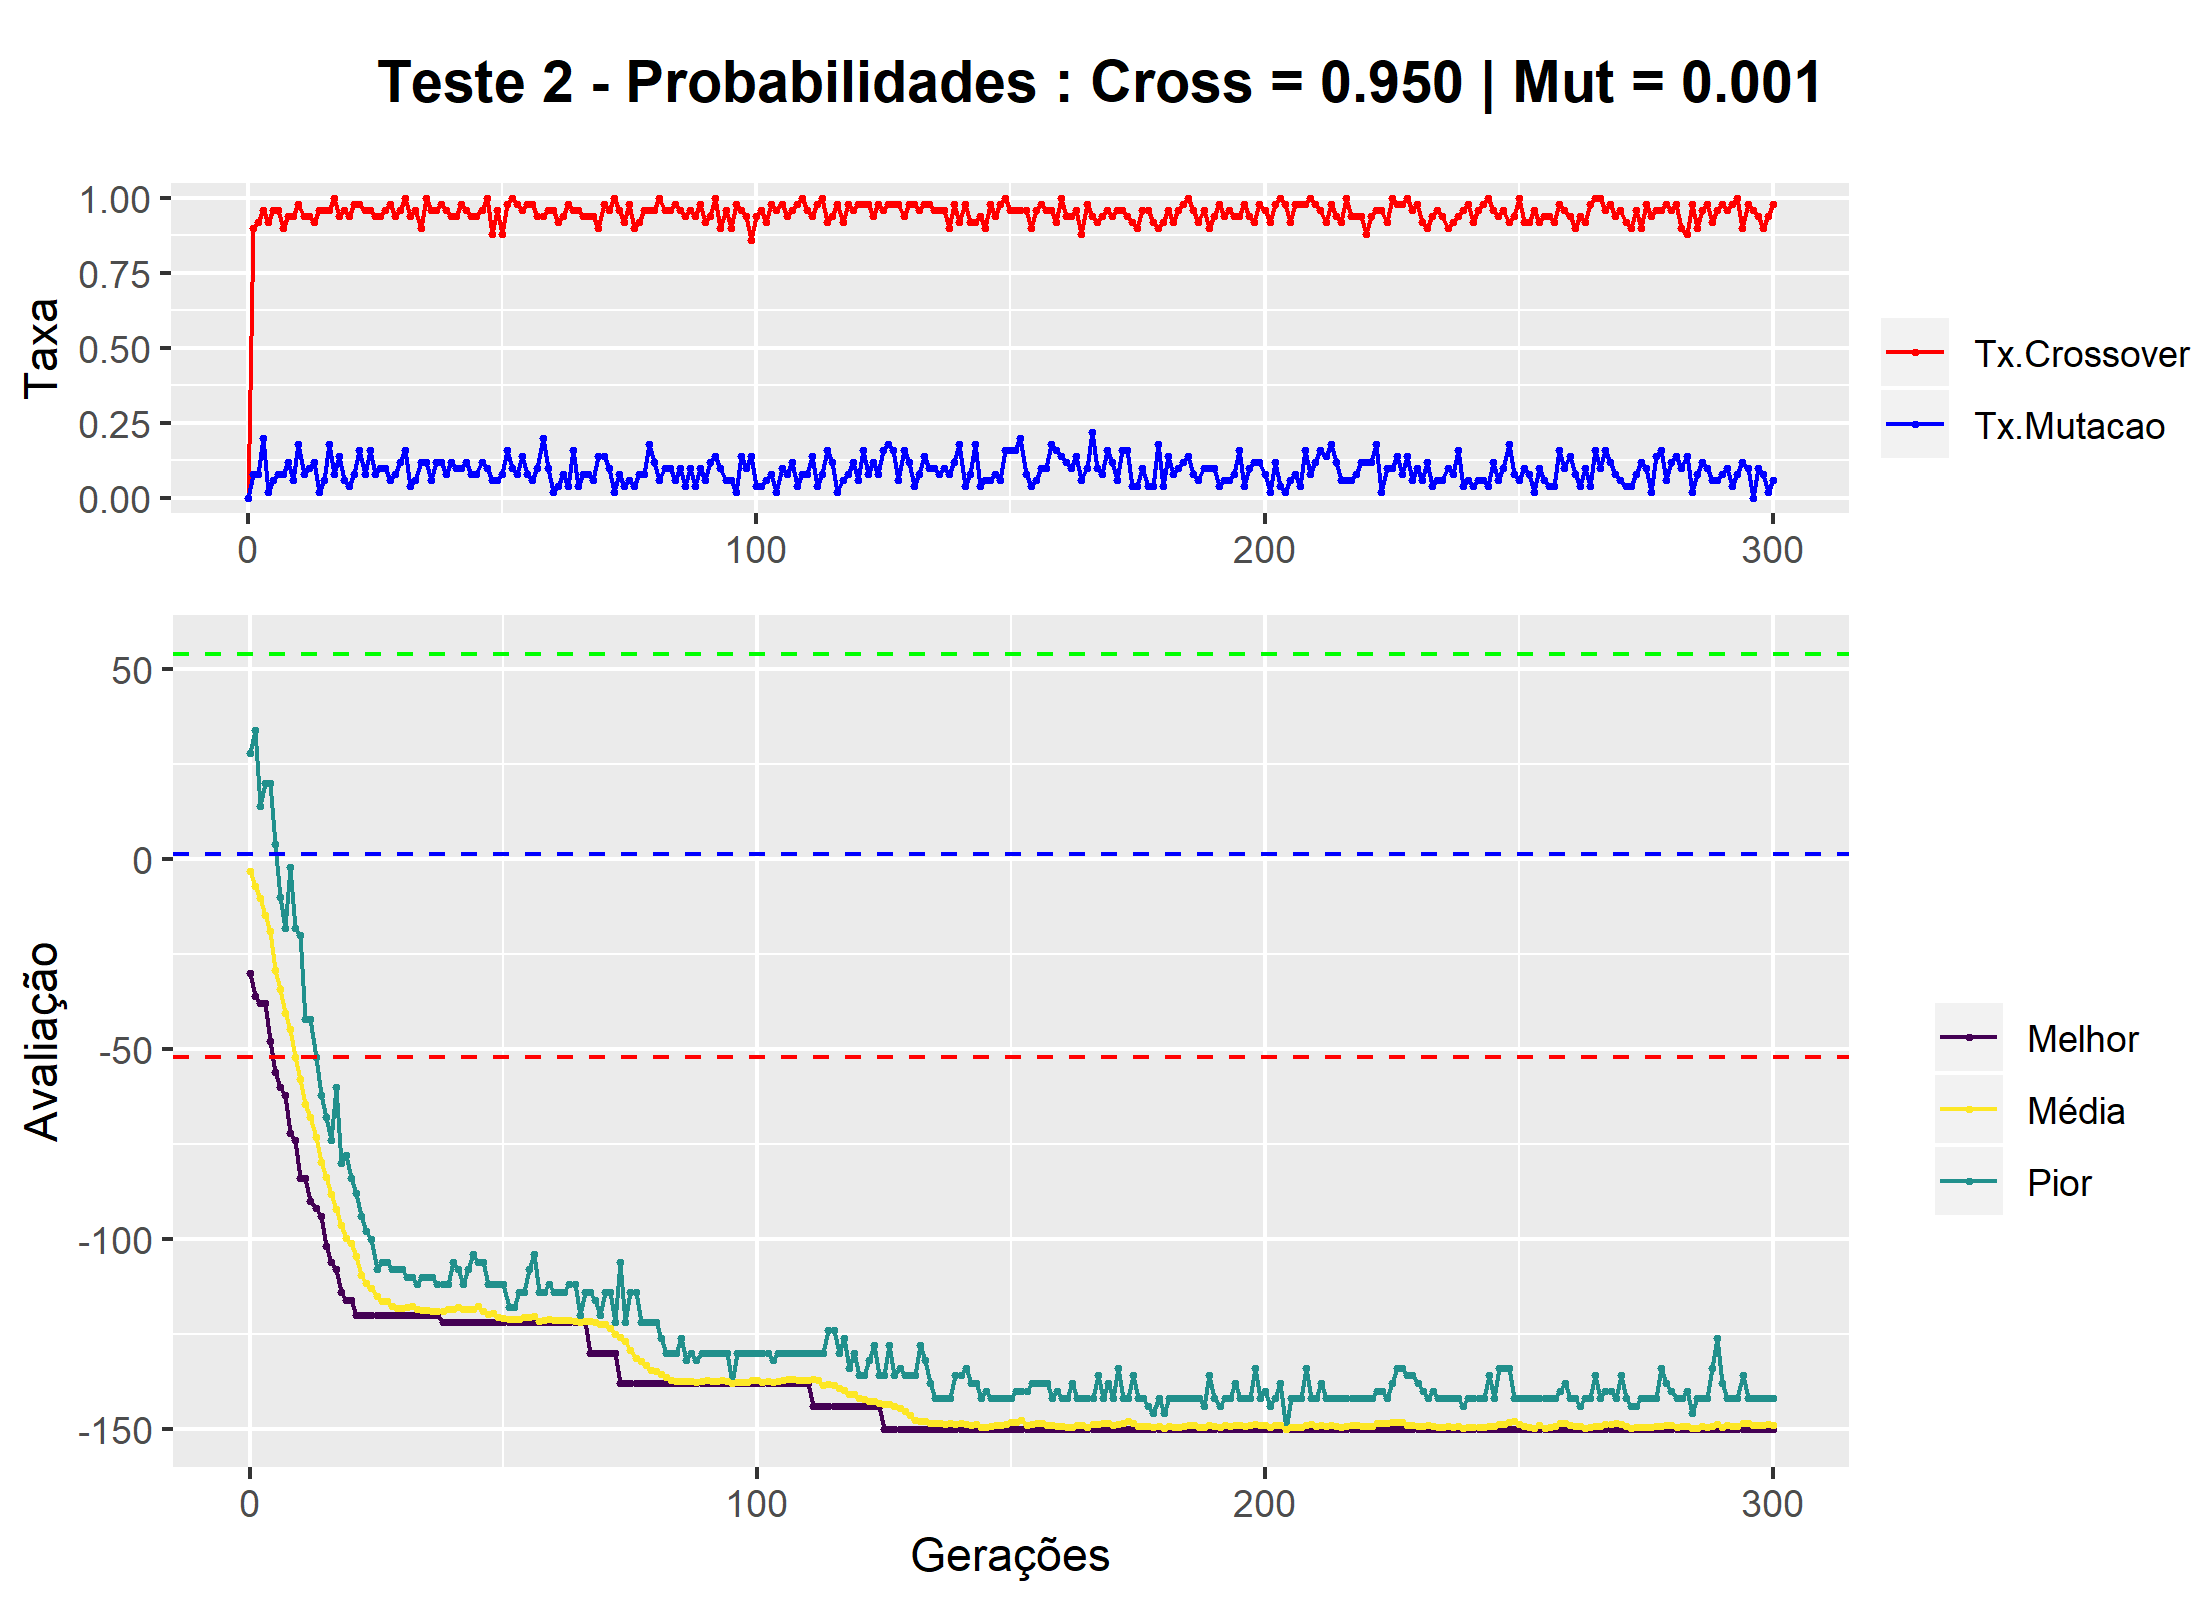
\includegraphics[width=\linewidth]{imagens/graph_pc_0_950_pm_0_001_pop_50_g_300__2.png}
		\caption{}
	\end{subfigure}
	\begin{subfigure}[b]{0.47\linewidth}
		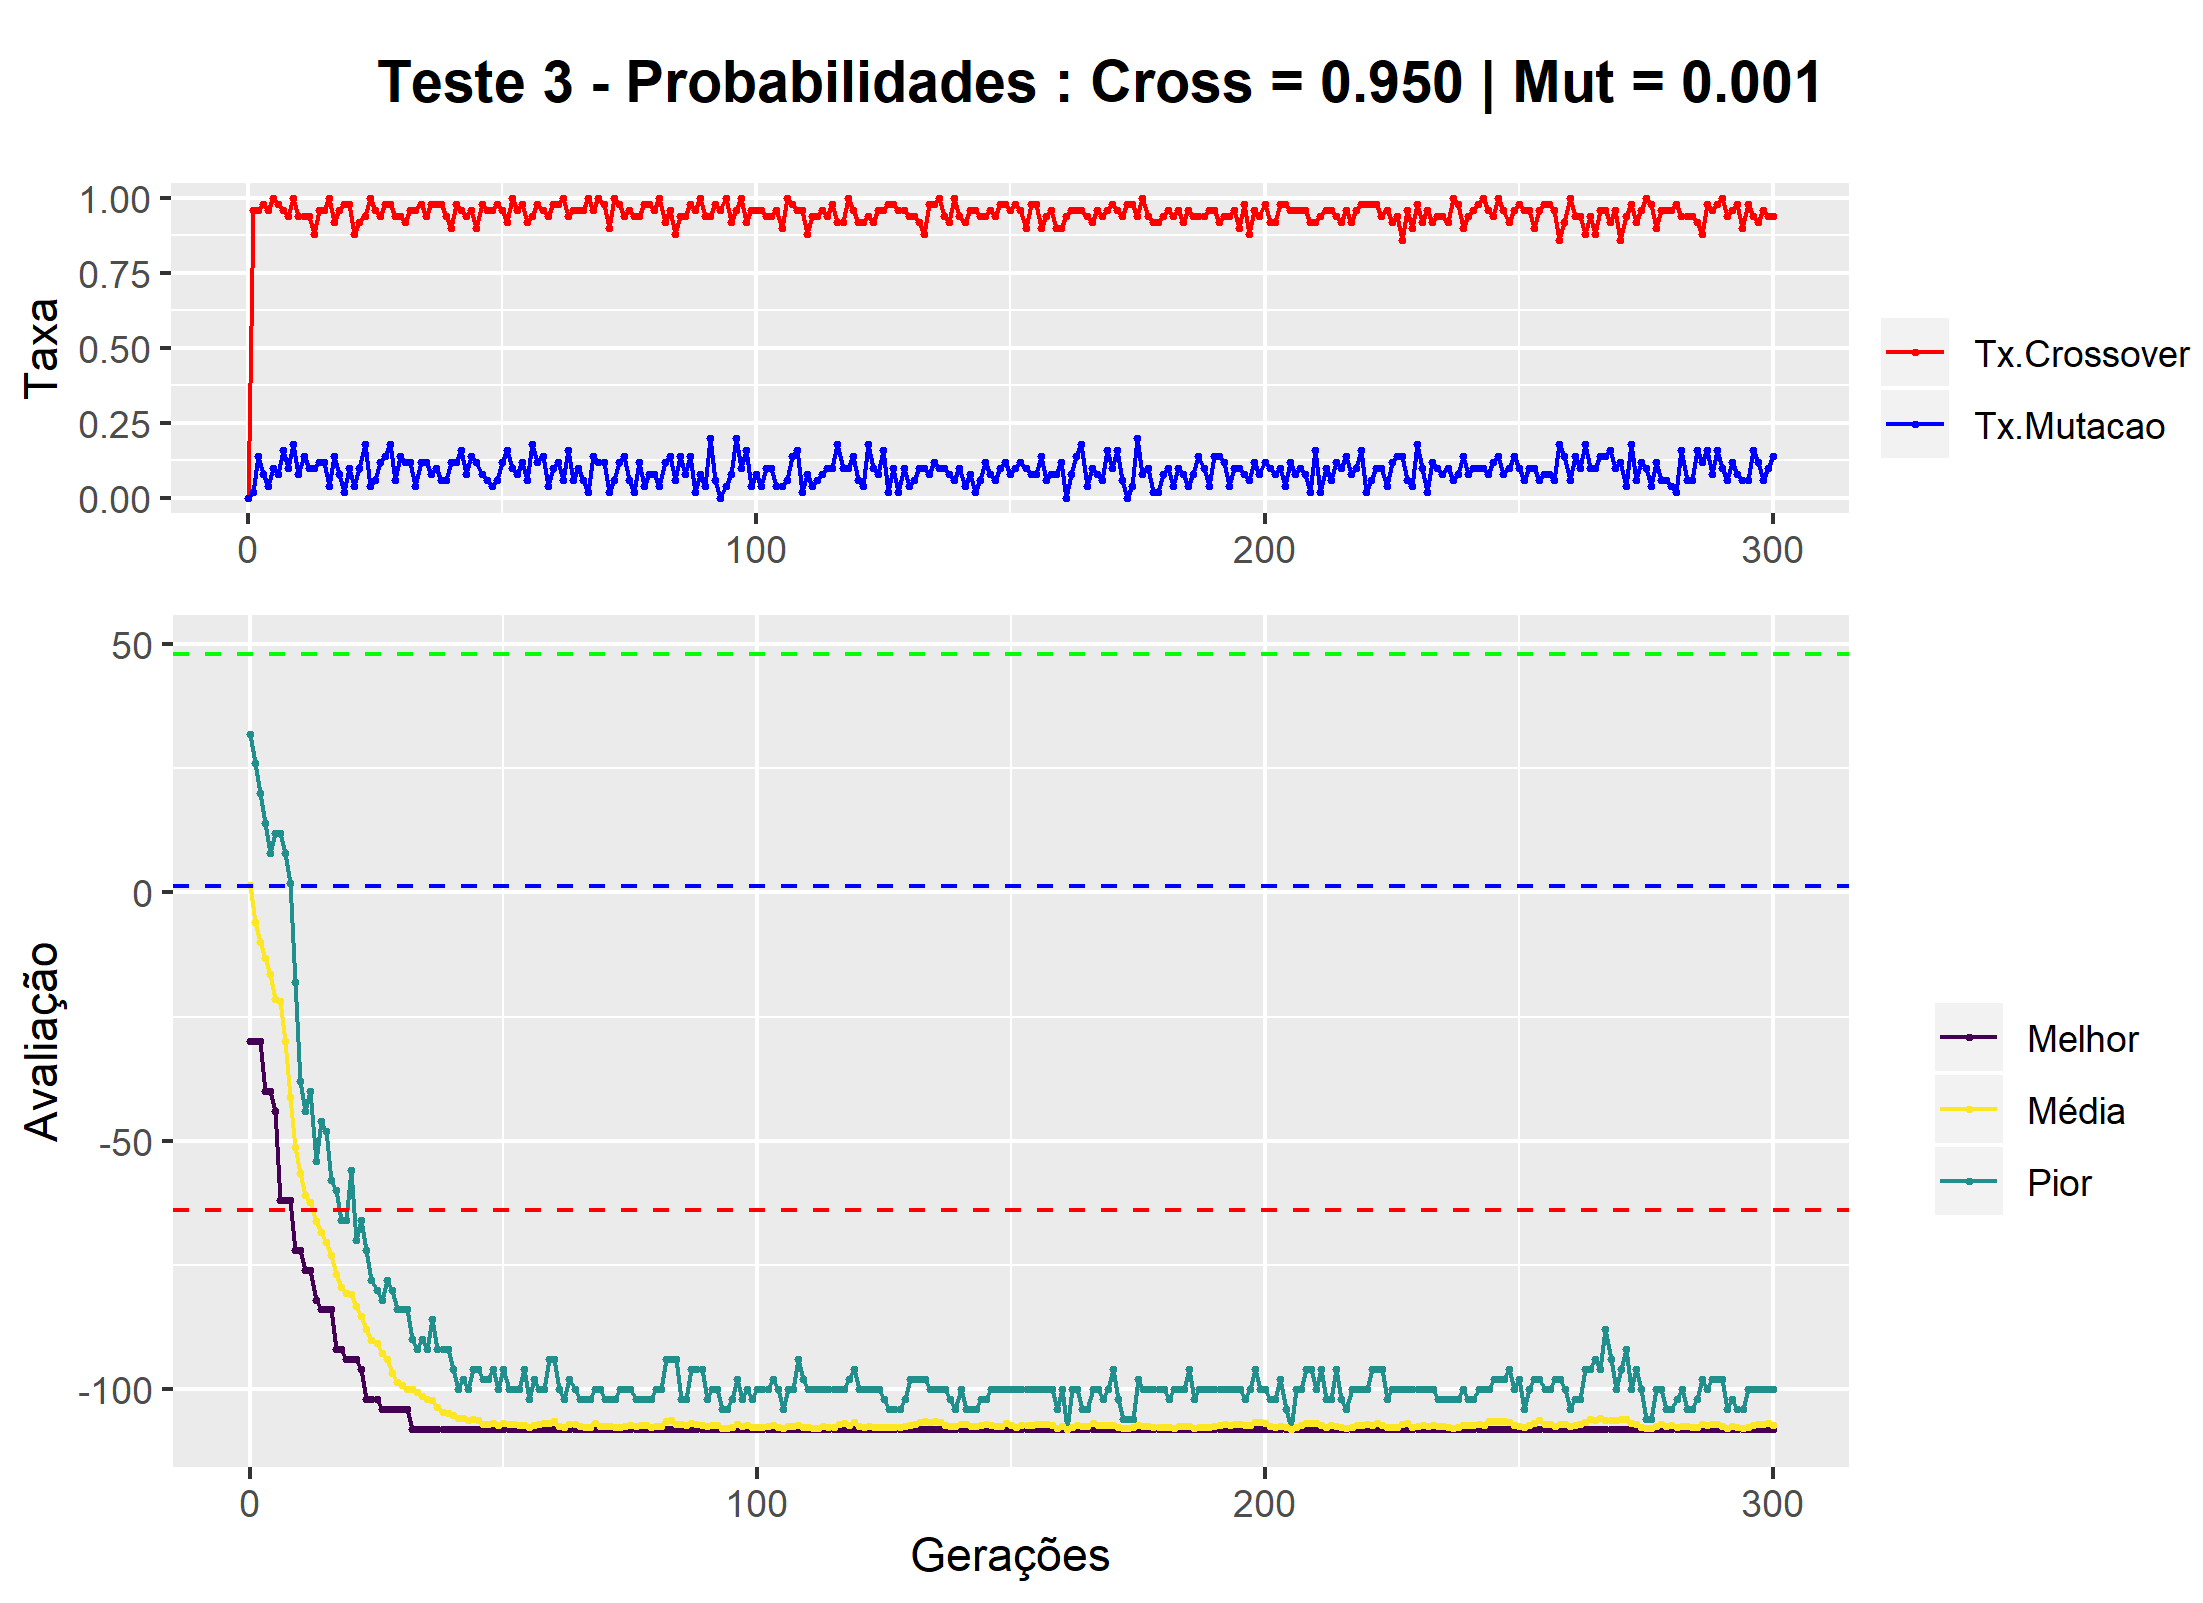
\includegraphics[width=\linewidth]{imagens/graph_pc_0_950_pm_0_001_pop_50_g_300__3.png}
		\caption{}
	\end{subfigure}
	\begin{subfigure}[b]{0.47\linewidth}
		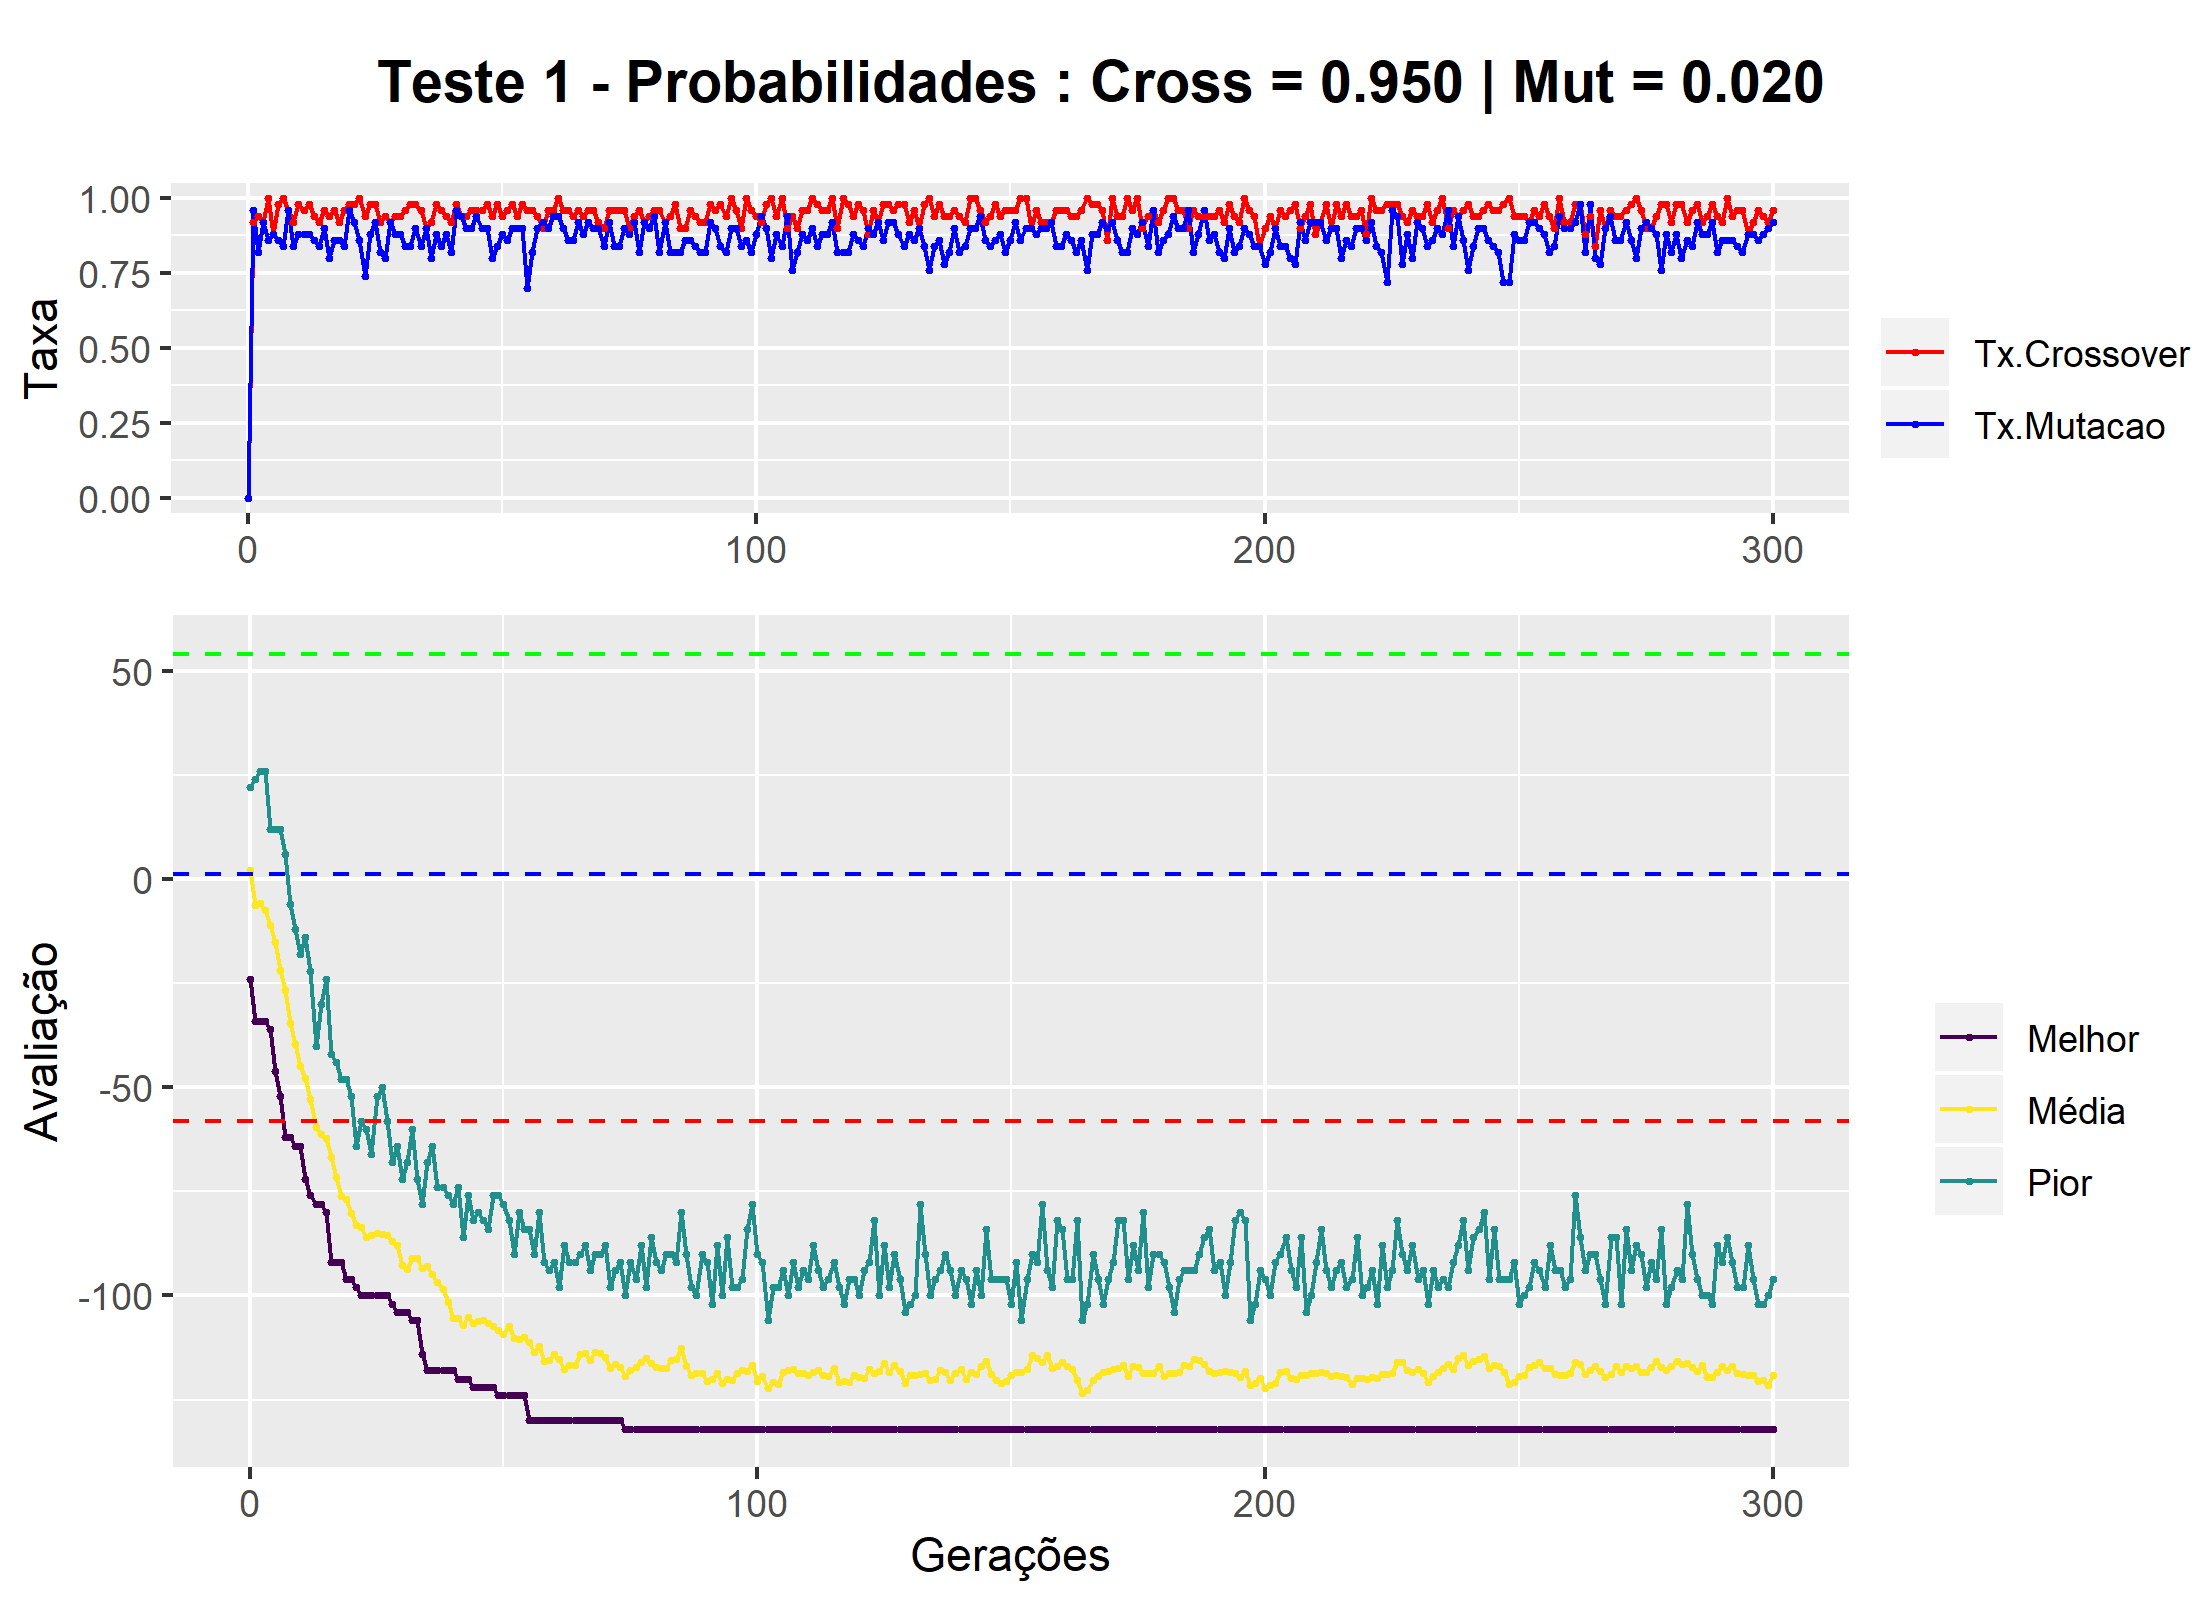
\includegraphics[width=\linewidth]{imagens/graph_pc_0_950_pm_0_020_pop_50_g_300__1.png}
		\caption{}
	\end{subfigure}
	\begin{subfigure}[b]{0.47\linewidth}
		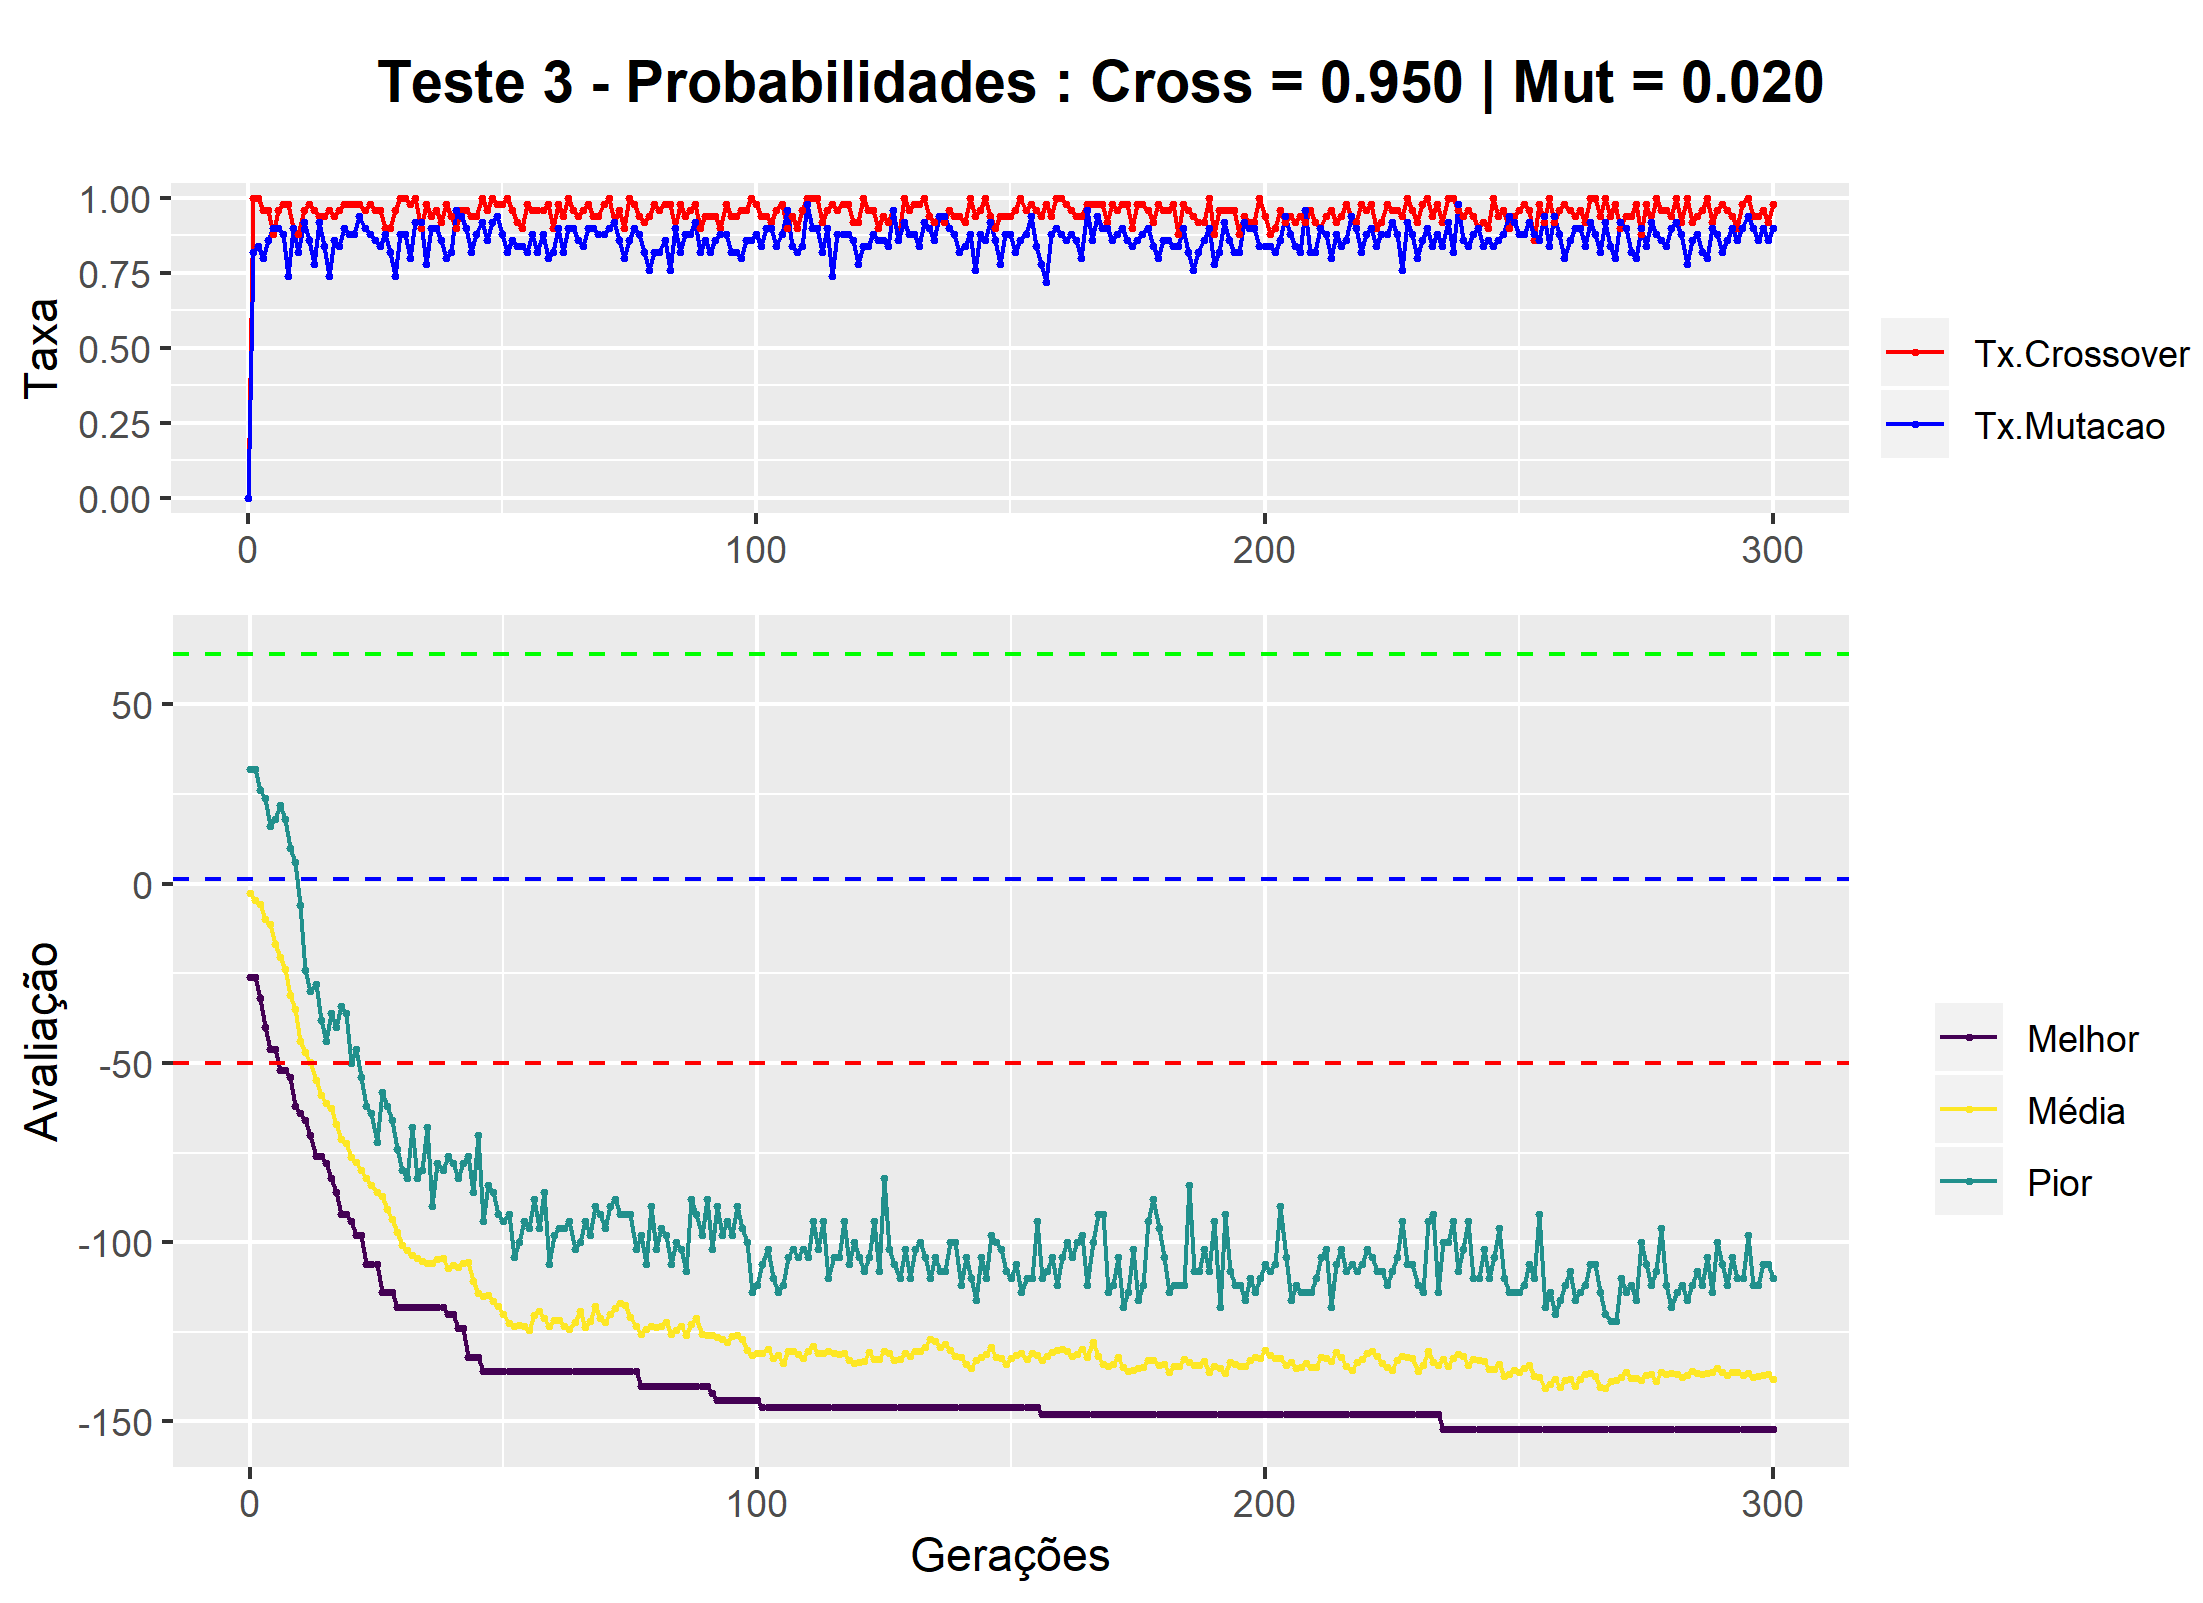
\includegraphics[width=\linewidth]{imagens/graph_pc_0_950_pm_0_020_pop_50_g_300__3.png}
		\caption{}
	\end{subfigure}
	\begin{subfigure}[b]{0.47\linewidth}
		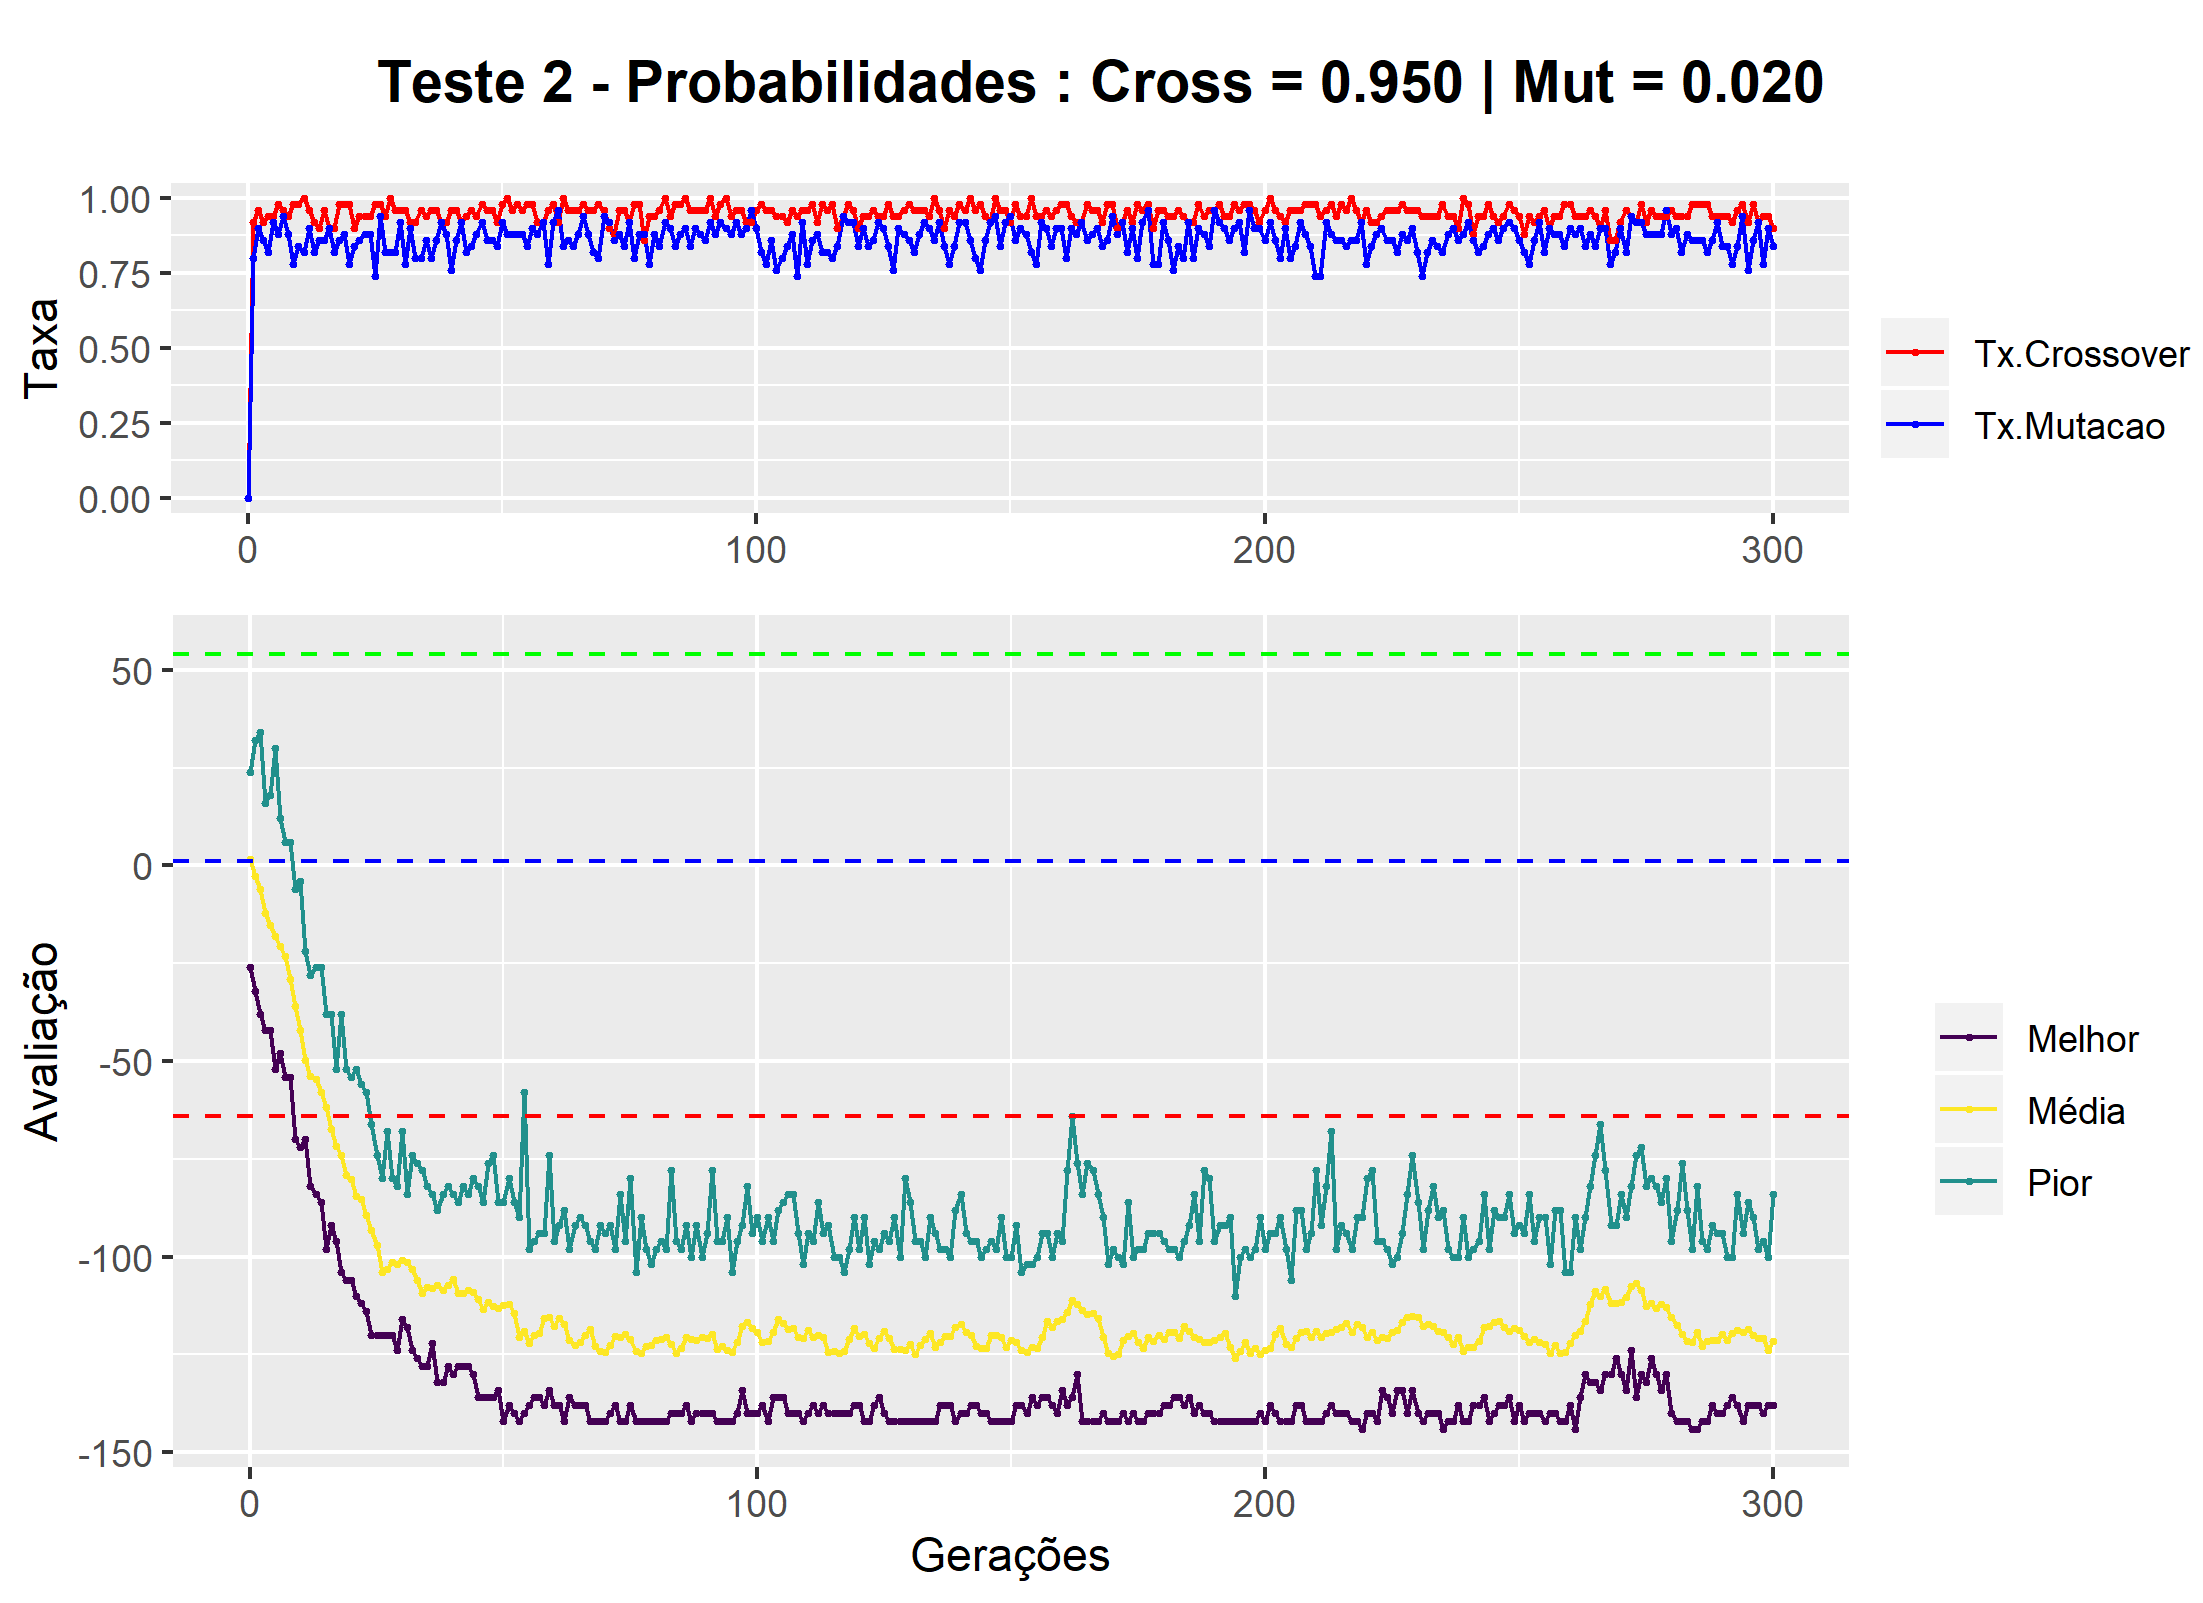
\includegraphics[width=\linewidth]{imagens/graph_pc_0_950_pm_0_020_pop_50_g_300__2_noelite.png}
		\caption{Sem elitismo}
	\end{subfigure}
	\begin{subfigure}[b]{0.47\linewidth}
		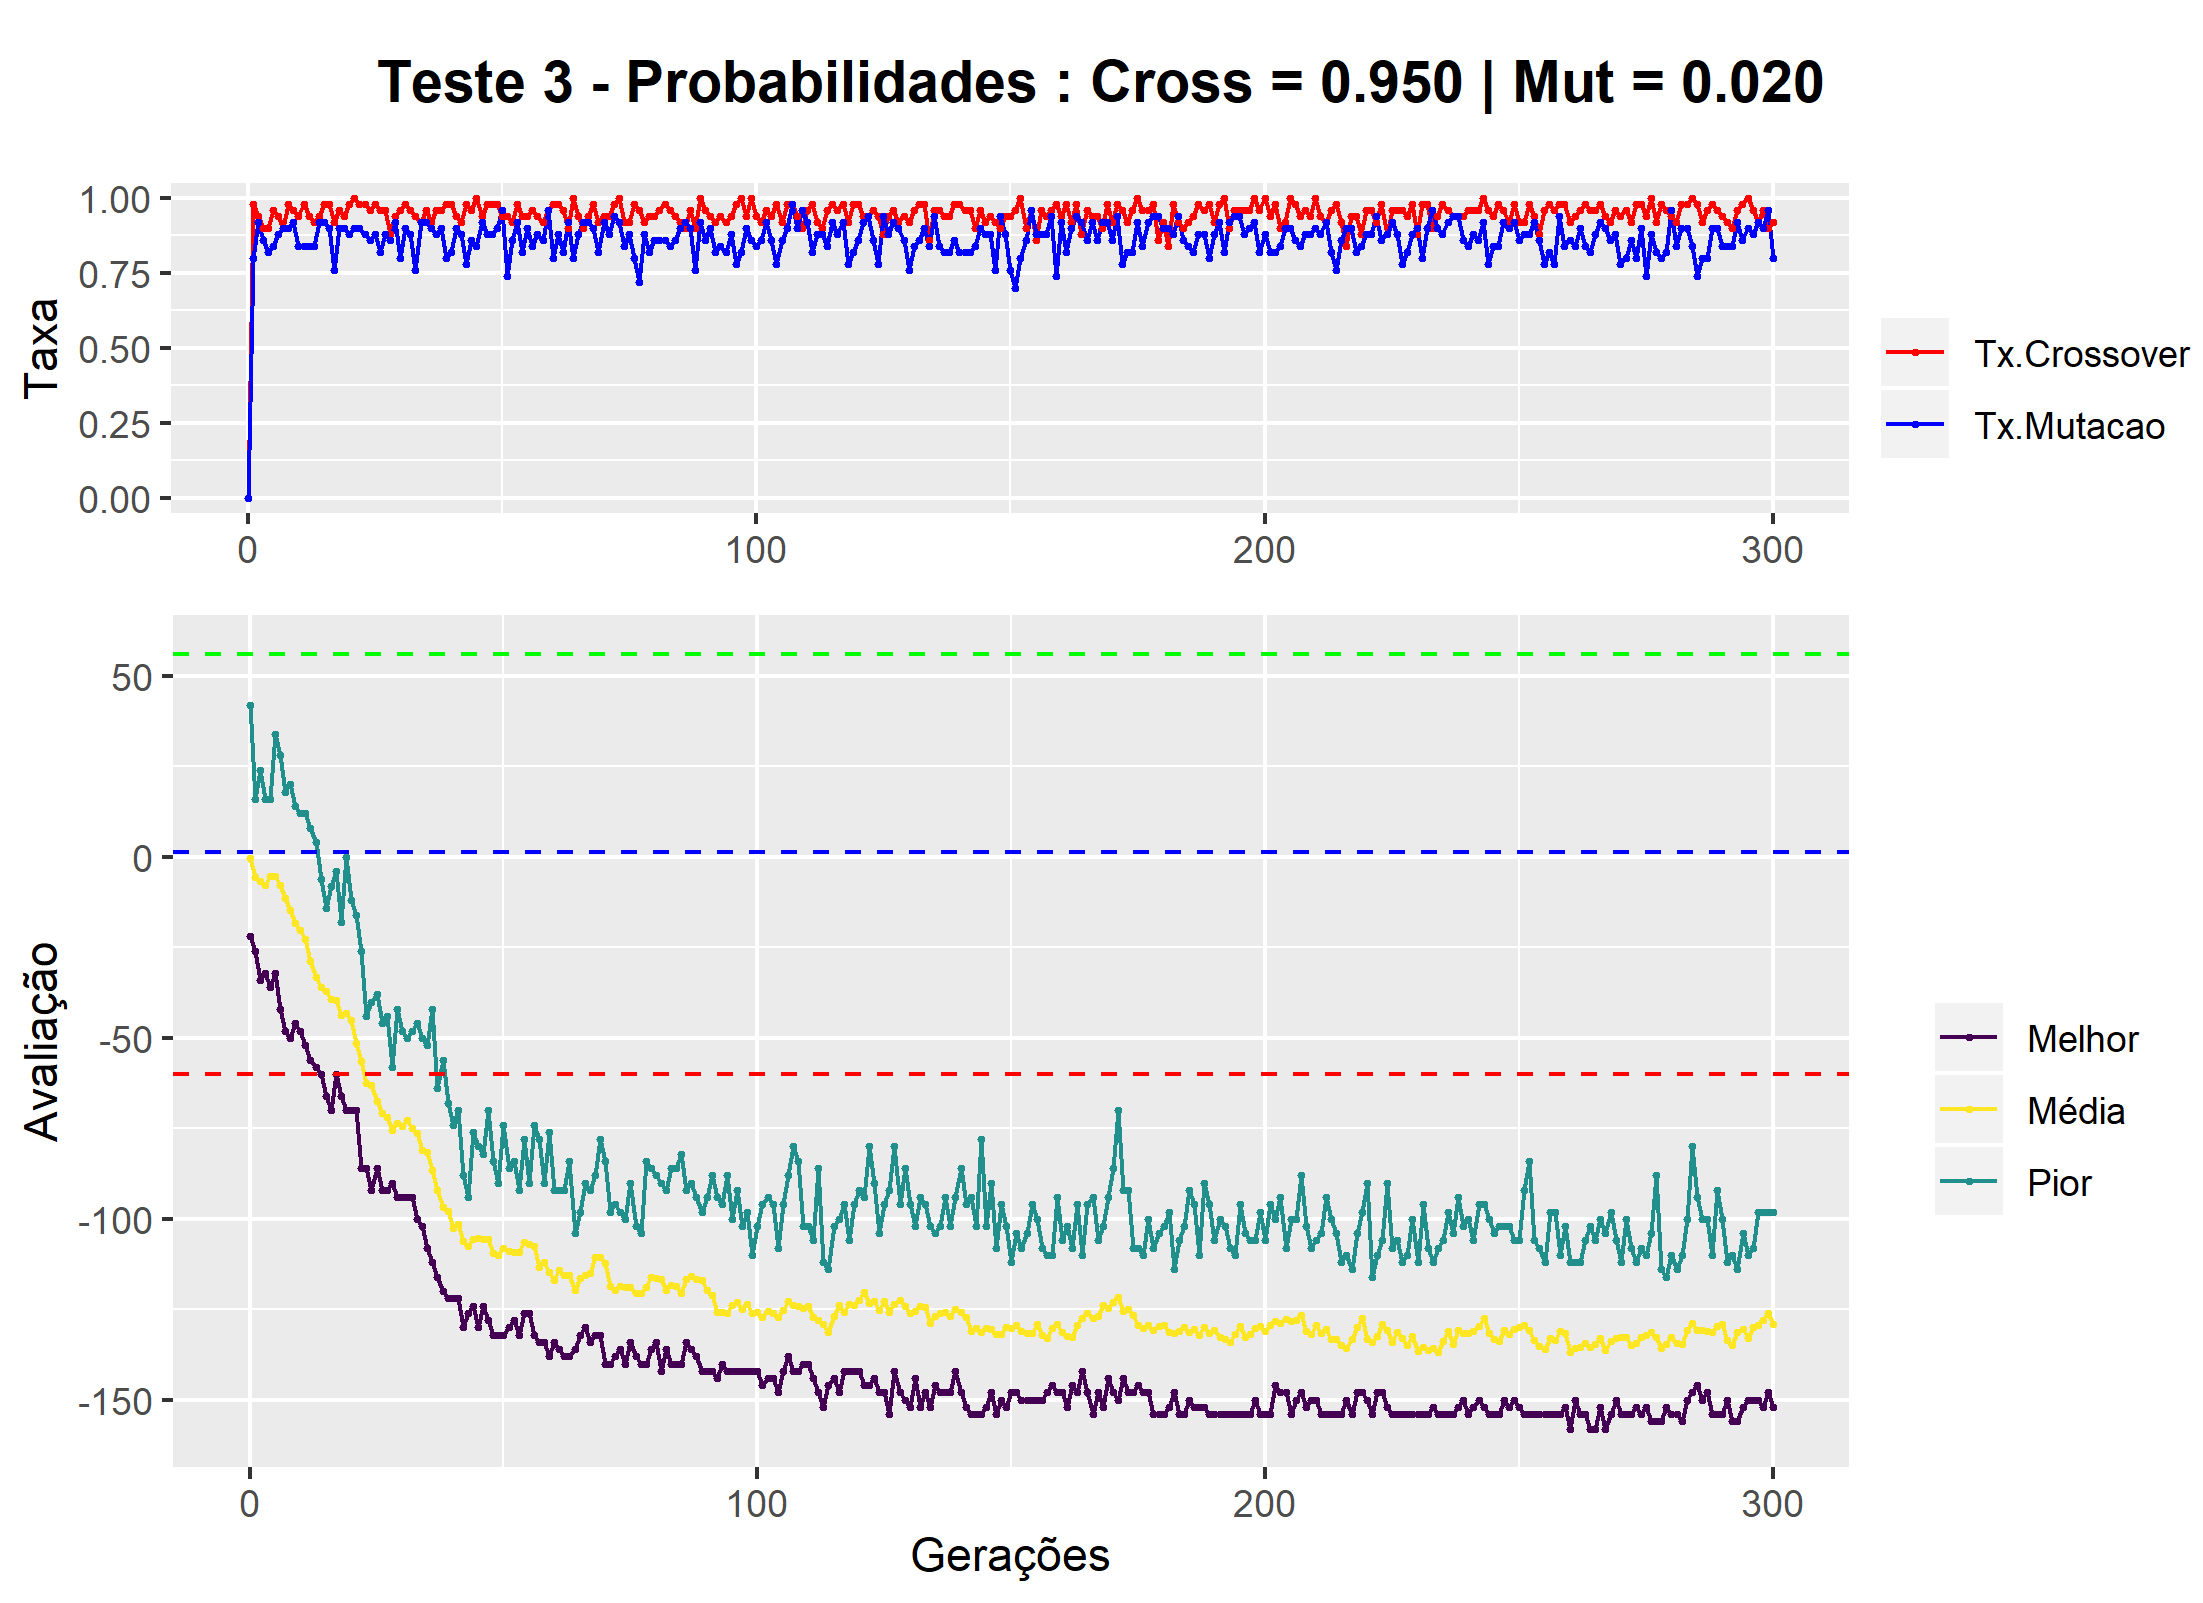
\includegraphics[width=\linewidth]{imagens/graph_pc_0_950_pm_0_020_pop_50_g_300__3_noelite.png}
		\caption{Sem elitismo}
	\end{subfigure}
	\caption{Evolução do algoritmo genético durante gerações}
	\label{fig:evolucaoGA2}
\end{figure}